\documentclass[a4paper,14pt]{extarticle} \usepackage[utf8]{inputenc}
\usepackage[T1]{fontenc}
\usepackage[margin=2.5cm]{geometry}

% Fonte Caladea se existir, senão lmodern
\IfFileExists{caladea.sty}{
  \usepackage{caladea}
}{
  \usepackage{lmodern} }
\usepackage{ragged2e}
\usepackage{graphicx}
\usepackage[portuguese]{babel}
\usepackage{wrapfig}
\usepackage{hyperref}
\usepackage{fancyhdr}
\usepackage{xcolor}
\usepackage{rotating}
\usepackage{titlesec}
\usepackage{epigraph}
\usepackage{dirtytalk}
\usepackage{indentfirst} % Indenta o primeiro parágrafo após seções

% Ajuste do recuo de parágrafo
\setlength{\parindent}{1.5em}

% Adjust headheight to remove LaTeX warning
\setlength{\headheight}{17.54163pt}

% Centralizar títulos
\titleformat{\section}
  {\normalfont\centering\bfseries\Large}{}{1em}{}

\titleformat{\subsection}
  {\normalfont\centering\bfseries\large}{}{1em}{}

\titleformat{\subsubsection}
  {\normalfont\centering\bfseries}{}{1em}{}

% -------------- Símbolos de Versículo e Resposta --------------
% Definição do símbolo (a “barrinha” inclinada)
\makeatletter
\newcommand{\vers@resp@sym}{%
  \raisebox{0.2ex}{\rotatebox[origin=c]{-20}{$\m@th\rceil$}}%
}
% macro interna que sobrepõe a barrinha e a letra V ou R
\newcommand{\vers@resp}[2]{%
  {\ooalign{%
     \hidewidth\kern#1\vers@resp@sym\hidewidth\cr
     #2\cr
  }}%
}
% comandos públicos \versicle e \response
\DeclareRobustCommand{\versicle}{\vers@resp{-0.1em}{V}}
\DeclareRobustCommand{\response}{\vers@resp{0pt}{R}}
\makeatother
% ^------------- Símbolos de Versículo e Resposta -------------^

% Rodapé com imagem e página
\pagestyle{fancy}
% ---- Cabeçalho ------------
\fancyhf[C]{}
% ----- Rodapé --------------
\fancyfoot[C]{%
  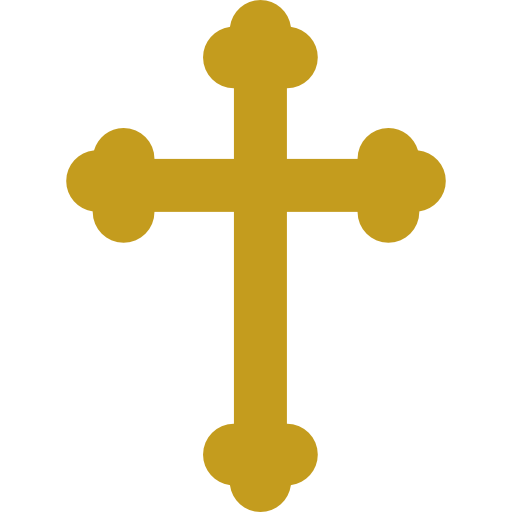
\includegraphics[scale=0.2]{assets/cross.png}\quad
  \textit{\textit{Santa Eusébia, Rogai por Nós}}\quad
  \thepage
}

\usepackage{pdfpages}
\begin{document}
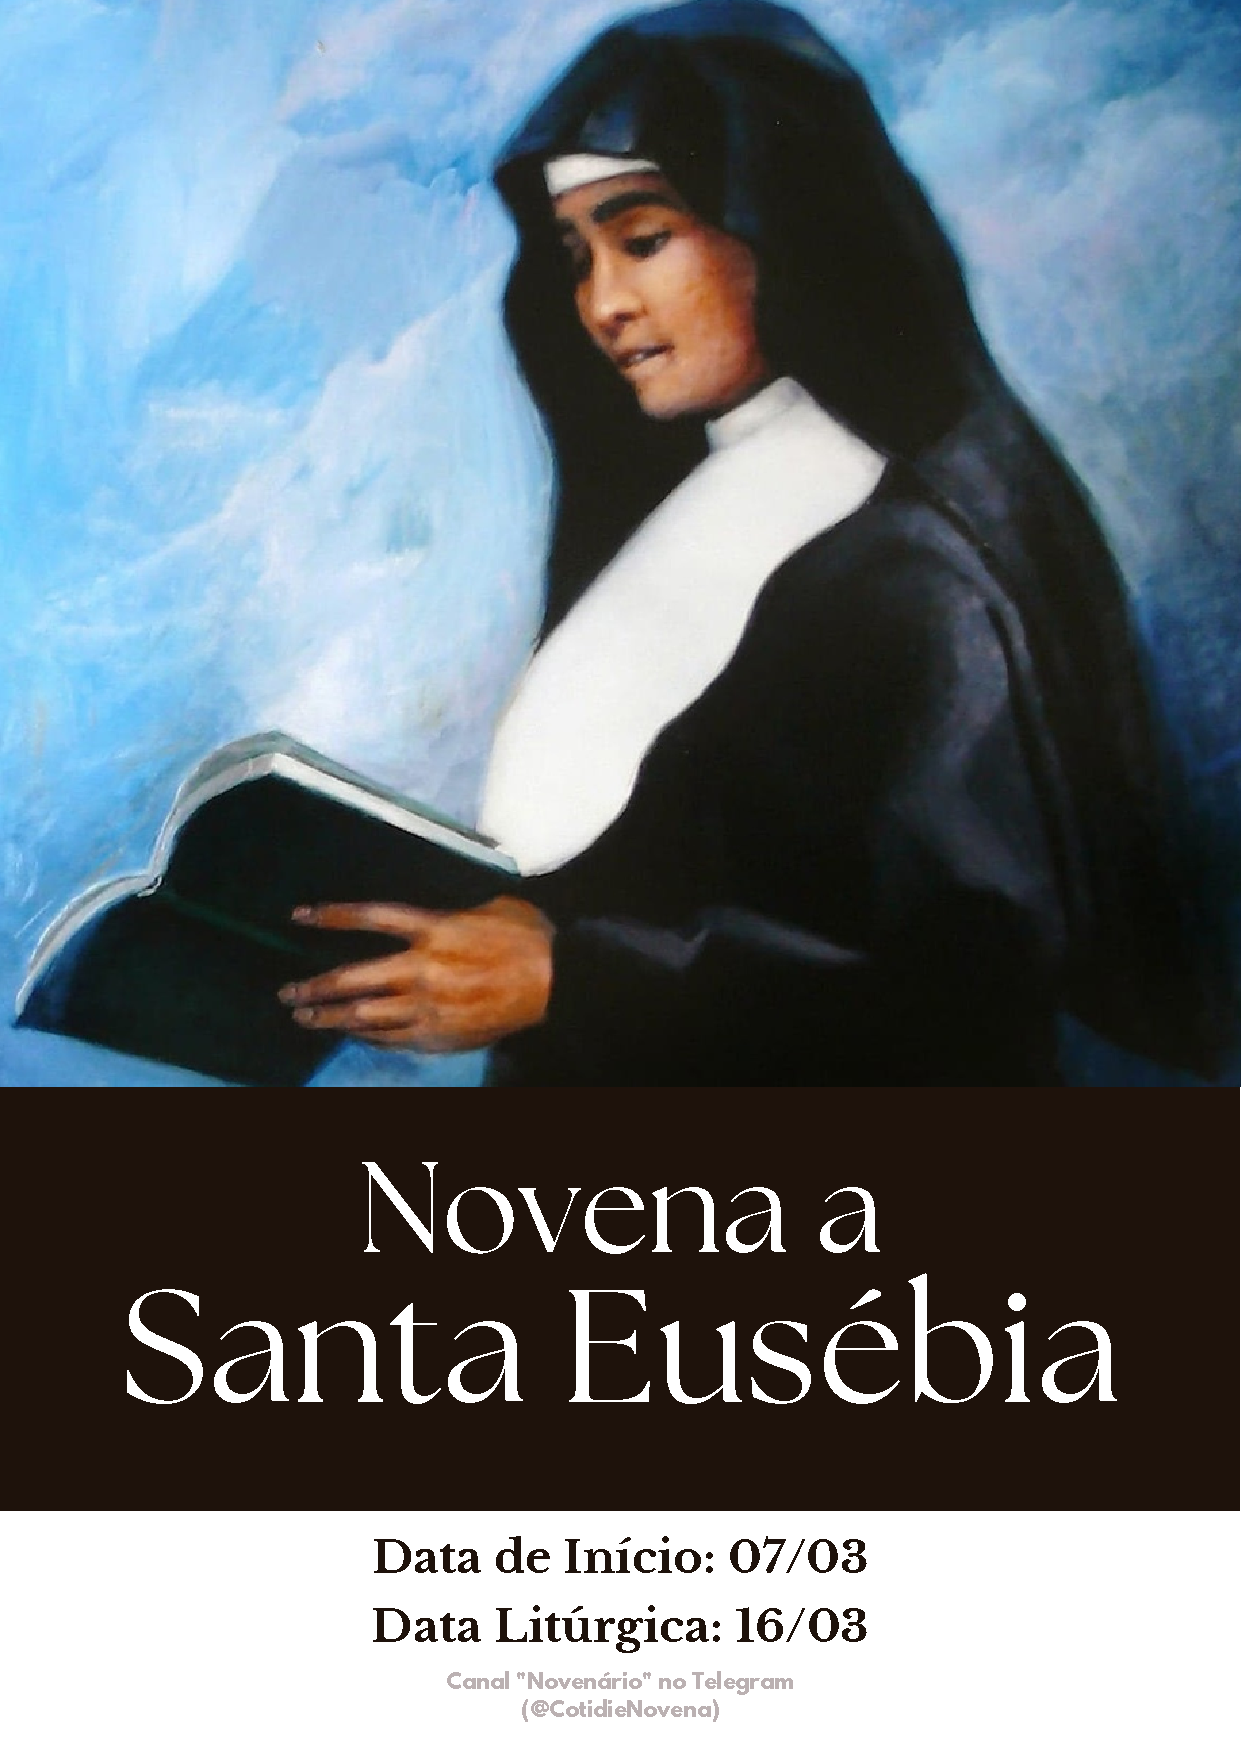
\includepdf[pages=1]{Capa Santa Eusébia.pdf}

\begin{center}
  {\huge Novena de Santa Eusébia}
\end{center}



\noindent\rule{\textwidth}{0.4pt}

\tableofcontents

\thispagestyle{empty}


% --- Origem ---
\newpage

\section{História}

\subsection{Origens e juventude}

Santa Eusébia nasceu na Gália, região correspondente à atual França, por volta do século VI, em uma época em que a Igreja consolidava sua presença entre os povos bárbaros convertidos ao cristianismo. Era filha de uma família cristã nobre, profundamente fiel à fé e à moral católica. Desde a infância, Eusébia revelou uma inclinação incomum à oração, à leitura das Sagradas Escrituras e à caridade.

A jovem cresceu em um ambiente profundamente marcado pela influência monástica. Inspirava-se nos exemplos das santas abadessas da época, como Santa Radegunda e Santa Genoveva de Paris, cujas virtudes femininas e liderança espiritual eram modelos de santidade.

\subsection{Vocação religiosa}

Ainda adolescente, Eusébia decidiu consagrar sua vida a Deus, recusando as propostas de casamento que lhe foram apresentadas. Seu coração pertencia ao Senhor, e sua alma ardia pelo ideal da vida consagrada. Com o consentimento dos pais, ingressou em um mosteiro da ordem beneditina, onde recebeu formação espiritual e teológica.

Ali, destacou-se pela humildade e pelo amor à Regra de São Bento, praticando com fidelidade a obediência e a pobreza. Em pouco tempo, tornou-se exemplo para as demais religiosas e foi escolhida para assumir responsabilidades dentro da comunidade.

\subsection{Abadessa de Hamay}

Após a morte de sua mãe, Santa Rictrudes, que também havia se tornado religiosa, Eusébia foi chamada a sucedê-la como abadessa do mosteiro de Hamay, situado na diocese de Cambrai, no norte da França. Tinha então apenas dezoito anos. Apesar da pouca idade, demonstrou extraordinária prudência, doçura e firmeza de espírito.

O mosteiro, sob sua direção, transformou-se em centro de vida espiritual e caridade. Eusébia organizou a rotina das monjas segundo os princípios da Regra beneditina, introduzindo períodos de silêncio, lectio divina e oração comunitária. Também se preocupava com a formação das jovens, vendo nelas futuras esposas de Cristo.

\subsection{Conflitos e provações}

A santidade de Eusébia, contudo, não a poupou das provações. Um dos parentes de sua mãe, Santo Mauronto, desejava transferir a comunidade de Hamay para outro local, acreditando que as jovens precisavam de orientação mais rígida. Eusébia, confiante em que a vontade de Deus se manifestaria pela paz, resistiu com serenidade, buscando o conselho dos bispos da região.

A disputa chegou a ser levada ao bispo de Cambrai, que reconheceu a legitimidade da abadessa e confirmou-a na direção do mosteiro. Com espírito obediente, Eusébia perdoou os que a criticaram e ofereceu suas lágrimas pela unidade da Igreja e pela santificação de suas irmãs.

\subsection{Modelo de virtude e mestra da fé}

A vida de Santa Eusébia foi um testemunho vivo da caridade evangélica. Passava longas horas em oração diante do altar, intercedendo pelas religiosas e pelos pobres da região. Não tolerava desperdícios nem luxo no mosteiro, insistindo que tudo fosse partilhado com os necessitados.

Era conhecida por sua voz suave e firme. Nas conferências espirituais, dizia às noviças:

"A alma que ama a Deus deve ser como o incenso: quanto mais é consumida, mais se eleva ao Céu."

Sua presença serena e maternal transformou o mosteiro num verdadeiro jardim de virtude. Mesmo os bispos locais consultavam-na em questões espirituais, reconhecendo nela sabedoria vinda do alto.

\subsection{Morte santa e culto}

Santa Eusébia faleceu por volta do ano 680, ainda jovem, depois de uma enfermidade prolongada que suportou com paciência heroica. Nos últimos dias, pediu que lhe lessem os Salmos penitenciais e que o crucifixo fosse colocado sobre o peito. Morreu recitando as palavras:

"Em vossas mãos, Senhor, entrego o meu espírito."

Seu corpo foi sepultado no próprio mosteiro de Hamay, que passou a ser lugar de peregrinação.

Numerosos milagres foram atribuídos à sua intercessão, especialmente curas de doenças infantis e reconciliações familiares.

O culto de Santa Eusébia foi aprovado pela Igreja no início da Idade Média. Em várias regiões da França e da Bélgica, ergueram-se igrejas sob sua invocação, e seu nome passou a figurar nos martirológios beneditinos.

\subsection{Espiritualidade e exemplo}

Santa Eusébia é lembrada como modelo de pureza, humildade e fortaleza. Sua vida demonstra que a verdadeira autoridade nasce da santidade e do amor. Embora tenha vivido em um tempo de grandes transformações políticas e religiosas, manteve-se fiel à oração e à vida interior.

Sua espiritualidade unia contemplação e ação: rezava com o mesmo fervor com que governava, e governava com a mesma serenidade com que rezava. Em todas as circunstâncias, via a vontade de Deus como guia supremo.

\subsection{Lições para o presente}

A figura de Santa Eusébia continua atual em uma época em que a vida consagrada é desafiada por dispersões e pela perda do sentido de sacrifício. Sua fidelidade à Regra, sua sensibilidade feminina e sua prudência pastoral revelam o equilíbrio perfeito entre firmeza e ternura.

Ela recorda que a santidade não se mede pela idade, mas pela fidelidade. Mesmo jovem, exerceu liderança espiritual que transformou sua comunidade num farol de fé.

\subsection{Representação e devoção}

Santa Eusébia é representada com hábito beneditino, segurando um livro - símbolo da Regra monástica - e um lírio branco, sinal de pureza. Às vezes, aparece também com um báculo de abadessa e um pequeno mosteiro aos pés, indicando sua missão de guia espiritual.

Sua festa litúrgica é celebrada em 16 de março, e seu nome é invocado especialmente por jovens religiosas e educadoras.

Na França e na Bélgica, diversas paróquias ainda guardam relíquias associadas a ela, e peregrinos visitam suas antigas fundações pedindo proteção para famílias e comunidades religiosas.

% --- Orações Diárias ---
\newpage

\vfill

\section{Orações}
\subsection{Oração Inicial}\label{sub:inicial} % (fold)

Ó Deus, que concedestes a Santa Eusébia a graça de seguir-Vos com coragem desde a juventude, concedei-nos, por sua intercessão, a força para vivermos uma vida de entrega total ao Vosso serviço. Que ela, que encontrou na clausura e na obediência o caminho da santidade, nos inspire a buscar a Vossa vontade acima de tudo.

Neste momento, apresento a Vós, Senhor, as minhas intenções:
\textit{Coloque aqui suas intenções...}



\subsection{1º Dia - O Chamado na Juventude}

\underline{\nameref{sub:inicial}}

Santa Eusébia, desde criança, foi educada na fé por sua mãe, Santa Rictrude. Aos 12 anos, entrou no mosteiro de Marchiennes, respondendo ao chamado de Deus com generosidade.
Ó Santa Eusébia, que abandonastes o mundo para seguir Cristo, ajuda-me a discernir minha vocação com clareza. Ensina-me a ouvir a voz de Deus mesmo nas pequenas decisões. Amém.


\underline{\nameref{sub:final}}

\subsection{2º Dia - A Vida Monástica}

\underline{\nameref{sub:inicial}}

Santa Eusébia encontrou no mosteiro um refúgio de paz e união com Deus. Sua vida de oração, silêncio e trabalho manual foi um testemunho de amor à regra monástica.
Ó Santa Eusébia, que encontrastes em Deus o sentido da vida, ensina-me a valorizar a oração e o silêncio interior. Ajuda-me a buscar a intimidade com o Senhor no cotidiano. Amém.


\underline{\nameref{sub:final}}

\subsection{3º Dia - A Obediência à Vontade Divina}

\underline{\nameref{sub:inicial}}

Santa Eusébia obedeceu ao desejo de sua mãe e de seus superiores, permanecendo no mosteiro mesmo quando sua família tentou trazê-la de volta ao mundo.
Ó Santa Eusébia, que viveste a obediência como caminho de santidade, ajuda-me a acolher a vontade de Deus com humildade. Ensina-me a renunciar aos meus desejos egoístas para seguir Cristo. Amém.


\underline{\nameref{sub:final}}

\subsection{4º Dia - A Devoção à Família Santa}

\underline{\nameref{sub:inicial}}

Santa Eusébia cresceu em uma família de santos: sua mãe, Santa Rictrude, e seus irmãos, Santos Mauronto, Clotsinda e Adalsinda. Sua vida mostra que a santidade pode florescer no lar.
Ó Santa Eusébia, que fostes inspirada pelo exemplo dos teus familiares, ajuda-me a ser uma luz de fé para minha família. Ensina-me a construir um lar onde Deus seja amado. Amém.


\underline{\nameref{sub:final}}

\subsection{5º Dia - A Humildade no Serviço}

\underline{\nameref{sub:inicial}}

Santa Eusébia, mesmo sendo abadessa, servia às irmãs com simplicidade. Ela lavava os pés das monjas e cuidava das doentes, imitando Cristo Servo.
Ó Santa Eusébia, que escolhestes o último lugar para glorificar a Deus, ensina-me a servir sem buscar reconhecimento. Ajuda-me a encontrar alegria nas pequenas tarefas do dia a dia. Amém.


\underline{\nameref{sub:final}}

\subsection{6º Dia - A Fidelidade nas Provações}

\underline{\nameref{sub:inicial}}

Santa Eusébia enfrentou conflitos familiares e pressões sociais, mas manteve-se fiel à sua consagração. Sua perseverança é um modelo para os que sofrem por causa da fé.
Ó Santa Eusébia, que resististes às tentações do mundo, ajuda-me a manter-me firme nas dificuldades. Concede-me a graça da perseverança final. Amém.


\underline{\nameref{sub:final}}

\subsection{7º Dia - O Amor à Castidade}

\underline{\nameref{sub:inicial}}

Santa Eusébia consagrou sua virgindade a Cristo, vivendo a castidade como um dom e uma oferta de amor. Sua pureza de coração brilhou como testemunho do Reino.
Ó Santa Eusébia, que guardastes a pureza como um tesouro, ajuda-me a viver a castidade segundo minha vocação. Ensina-me a amar com um coração livre e puro. Amém.


\underline{\nameref{sub:final}}

\subsection{8º Dia - A Morte como Encontro com o Esposo}

\underline{\nameref{sub:inicial}}

Santa Eusébia partiu para o céu ainda jovem, por volta dos 33 anos, após uma vida de entrega total. Sua morte foi um encontro jubiloso com Cristo, seu Esposo.
Ó Santa Eusébia, que entrastes na glória celeste em plena juventude, ajuda-me a viver cada dia como preparação para a eternidade. Concede-me a graça de uma morte santa. Amém.


\underline{\nameref{sub:final}}

\subsection{9º Dia - O Legado de Santidade}

\underline{\nameref{sub:inicial}}

Santa Eusébia deixou um legado de fé para a Igreja, inspirando gerações a buscar a Deus na vida contemplativa. Sua memória é celebrada como farol de santidade.
Ó Santa Eusébia, que hoje intercedeis por nós no céu, ajuda-me a ser um exemplo de fé para os outros. Ensina-me a deixar um rastro de amor e fidelidade ao Evangelho. Amém.


\underline{\nameref{sub:final}}

\subsection{Oração Final}\label{sub:final} % (fold) \subsection{Orações de Cada Dia}

\[\textbf{Pai-Nosso, Ave-Maria, Glória}\]

Ó Deus, que fizestes de Santa Eusébia um modelo de obediência, pureza e amor à vida monástica, concedei-nos, por sua intercessão, a graça de imitar suas virtudes. Que ela, que soube amar-Vos acima de todas as coisas, nos inspire a buscar a santidade em nossa vocação.

Lembrai-Vos, Senhor, das minhas intenções e concedei-me as graças que Vos peço, para a Vossa glória e o bem da minha alma. Por Cristo, Nosso Senhor. Amém.


\vfill

\begin{center}
\subsection*{Fontes:}
Adaptado de: {\color{blue} \underline{\href{https://cruzterrasanta.com.br/santa-eusebia/615/102/}{Cruz Terra Santa}}} e {\color{blue} \underline{\href{https://www.youtube.com/playlist?list=PLN7jQwkJvdQqZ3TDirRd2ygYI5ns92DhF}{Canal A Oração dos Santos}}}
\end{center}


\end{document}
